\documentclass[12pt,a4paper]{article}

\usepackage[T1]{fontenc}
\usepackage{amsmath, amssymb, amsfonts}
\usepackage[magyar]{babel}
\usepackage[utf8]{inputenc}
\usepackage{graphicx}
\usepackage{graphics}
\usepackage{mathtools}
\usepackage{epsfig}
\usepackage{epstopdf}
\usepackage{cite}
\usepackage{caption}
\usepackage{hyperref}
\usepackage[bottom=4cm]{geometry}
%\geometry{a4paper, portrait, margin=1in}

\title{\huge{Korszerű vizsgálati módszerek labor jegyzőkönyv}\\ \vspace{20pt}
\textbf{Magspektroszkópiai vizsgálatok} \\}

\author{\Large{\textsc{Csörnyei Géza}} \vspace{10pt}\\
	\textrm{Eötvös Loránd Tudományegyetem}\\
	\textrm{Fizika BSc III. évfolyam}
	}
\date{}
%\lhead{}
\begin{document}
\addtolength{\voffset}{-1.5cm}
\addtolength{\textheight}{1.5cm}
\begin{titlepage}
\maketitle

\begin{figure}[!htb]
\centering
  
\includegraphics[scale=0.6]{eltecimer.jpg}
\end{figure}

\hfil \Large{'C' mérőcsoport}\hfil  \\
\vspace*{2pt}
\hfil \Large{\emph{Mérés dátuma:} 2018.03.22.}\hfil \\
\vspace*{2pt}
\hfil \hspace*{45pt} \Large{\emph{Mérés vezetője:} Pávó Gyula}\hfil
\thispagestyle{empty}
\end{titlepage}

\section{Gamma spektroszkópia}
\subsection{Szcintillációs detektor}
\hspace*{10pt} A gamma spektroszkópiai vizsgálatainkat a szcintillációs detektor kalibrálásával kezdtük. Erre azért volt szükség, mert a spektrumokat sokcsatornás analizátor segítségével vettük fel, melynek csatornáihoz a kalibráció segítségével tudtunk energiatartományokat párosítani. A kalibráció során a spektrumokban látható egyes ismert energiájú csúcsokat Gauss-görbével illesztettem, melynek illesztéshez használt alakja:
$$f(x)=A\cdot e^{-\frac{(x-\mu)^2}{2\cdot \sigma ^2}} + c  .$$
A $c$ tagot a kontinuumszint figyelembevétele miatt kellett hozzáadnunk a görbéhez. A kalibrációhoz az illesztett görbék közepét (átlagát) kellett vennünk, és kellett összevetnünk a csúcsok ismert energiaértékeivel. A vizsgálat során felvett spektrumok at \ref{fig:1} ., míg az illesztések az \ref{fig:2} . és a \ref{fig:3} . ábrákon láthatók.\\
\begin{figure}[!h]
\centering
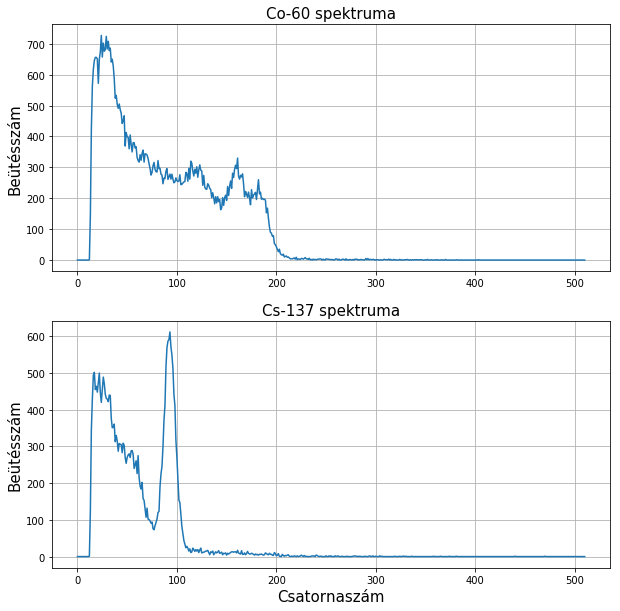
\includegraphics[scale=0.60]{szc_spekt}
\caption{A szcintillációs detektorral 120 s hosszú méréssel kapott spektrumok}
\label{fig:1}
\end{figure}
\newpage
\begin{figure}[!h]
\hspace*{-0.75cm}
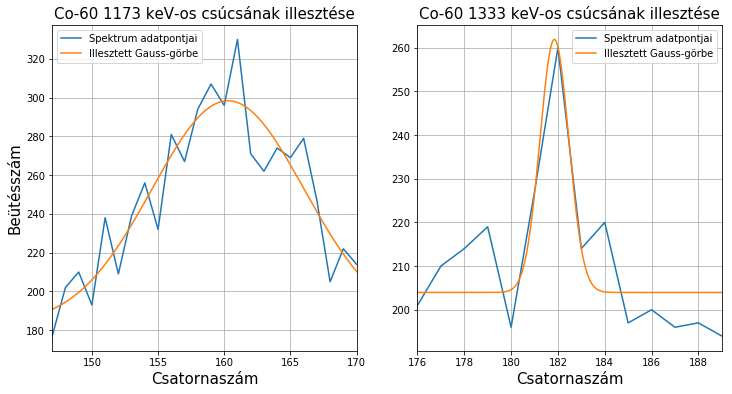
\includegraphics[scale=0.60]{Cob_figs}
\caption{A kobalt spektrumában látható első (1173 keV) és második (1333) csúcs illesztése}
\label{fig:2}
\end{figure}

Az illesztési paraméterek a fenti függvényalaknak megfelelő jelölésekkel:
\begin{table}[!h]
\begin{center}
\begin{tabular}{|c|c||c|}
\hline
Energia & 1173 keV & 1333 keV \\ 
\hline
$A$ & $115.619 \pm 18.067$ & $57.927 \pm 11.078$\\
\hline
$\mu$ & $160.286 \pm 0.400$ & $181.849 \pm 0.171$\\
\hline
$\sigma$ & $5.740 \pm 1.090$ & $0.616 \pm 0.139$ \\
\hline
$c$ & $182.754 \pm 19.411$ & $203.965 \pm 3.019$\\
\hline
\end{tabular}
\caption{A kobalt spektrumában látható csúcsok illesztési paraméterei}
\end{center}
\end{table}

\newpage

\begin{figure}[!h]
\centering
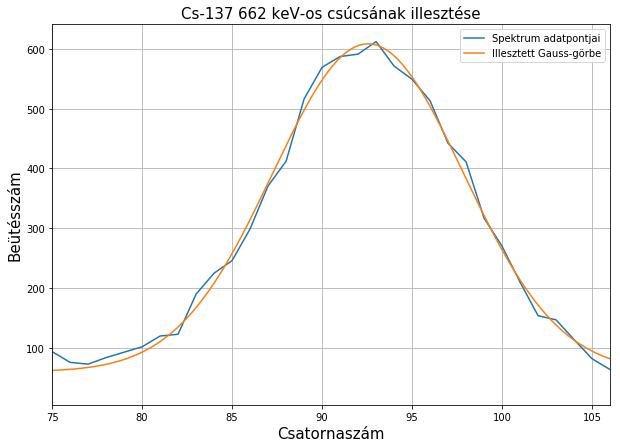
\includegraphics[scale=0.60]{Cs137_1csucs}
\caption{A cézium spektrumában látható csúcs (662 keV) illesztése}
\label{fig:3}
\end{figure}
Az illesztési paraméterek:
\begin{table}[!h]
\begin{center}
\begin{tabular}{|c|c|}
\hline
Energia & 662 keV \\ 
\hline
$A$ & $547.931 \pm 8.419$\\
\hline
$\mu$ & $92.557 \pm 0.076$\\
\hline
$\sigma$ & $5.291 \pm 0.117$\\
\hline
$c$ & $60.276 \pm 6.702$\\
\hline
\end{tabular}
\caption{A cézium spektrumában látható csúcs illesztési paraméterei}
\end{center}
\end{table}

\newpage
A kalibráció szempontjából fontos mennyiség számunkra a csúcsok helye, azaz a csatornaszám, melyen az illesztett Gauss-görbe átlaga van. Ezen értékek, valamint a csúcsokhoz tartozó energiaértékek ismeretében el tudjuk végezni a kalibrálást egyenesillesztés képében, mely a \ref{fig:4} . ábrán látható.

\begin{figure}[!h]
\centering
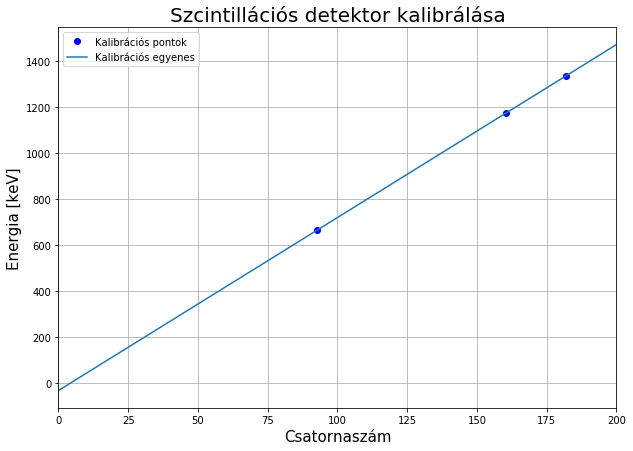
\includegraphics[scale=0.60]{Szcint_kalib}
\caption{A szcintillációs detektor kalibrálásához készített egyenesillesztés}
\label{fig:4}
\end{figure}

Az illesztett egyenes egyenlete:
$$ E(x) = 7.522 \cdot x - 33.903 ,$$
ahol $x$ a csatornaszámot jelöli, valamint mind a két oldal keV egységekben értendő.\\
\hspace*{10pt} A kalibráció elvégzése után lehetőségünk nyílt a detektor felbontóképességének meghatározására. Ehhez a $^{60}$Co 1333 keV-os csúcsának félértékszélességét számítottuk ki, ugyanis ez jól jellemezte a detektor felbontóképességét. Ennek oka, hogy csúcs mindössze egyetlen csatornában mért kiugró beütésszám értékként jelent meg, a szomszédos csatornákban már a kontinuumszinthez hasonló értékeket lehetett mérni. A félérték szélesség számításához az [1]-ben leírtaknak megfelelően lehet eljárni, azaz keV-ben mérve a félértékszélességet közelítőleg az 
$$ \Delta x = 2.36 \cdot \sigma $$
képlet határozza meg, ahol $\sigma$ az illesztett Gauss-görbe szórása. Ennek értelmében a fentebb említett mérés felhasználásával a mért félértékszélességre $ \Delta x = (10.934 \pm 2.475)$ keV adódik.\\
\newpage
A szcintillációs detektor segítségével felvettük egy NaCl (háttér) és egy KCl minta spektrumát is, majd meghatároztuk az ezekben vett $^{40}K$ intenzitás arányát. A felvett spektrumok a \ref{fig:5} . ábrán láthatók.
\begin{figure}[!h]
\centering
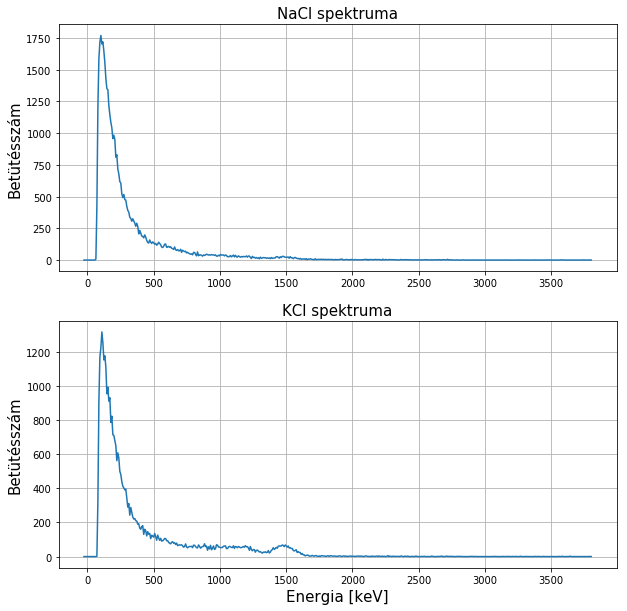
\includegraphics[scale=0.60]{Na-K_spek}
\caption{NaCl és KCl mintákkal felvett spektrumok}
\label{fig:5}
\end{figure}
\newline
A $^{40}$K-hez tartozó csúcsok és azok illesztései a két spektrum esetében a \ref{fig:6} . ábrán láthatók. Mivel a csúcs környékén a kontiunnum nem volt állandó értékkel közelíthető, ezért a csúcsok illesztése során a Gauss-görbét az alábbi módon egészítettük ki:
$$f(x)=A\cdot e^{-\frac{(x-\mu)^2}{2\cdot \sigma ^2}} + cx + b  .$$
A csúcsok intenzitásának arányánál az amplitúdóikat vetettük össze, ez azonban nem egyezik meg az illesztés során használt $A$-val, a Gauss-görbe definíciójából adódóan. Ennek megfelelően
$$A=A^{*}\frac{1}{\sqrt{2\pi \sigma}},$$
ahol $A^{*}$ az általunk használni kívánt amplitúdó érték.
\newpage
\begin{figure}[!h]
\centering
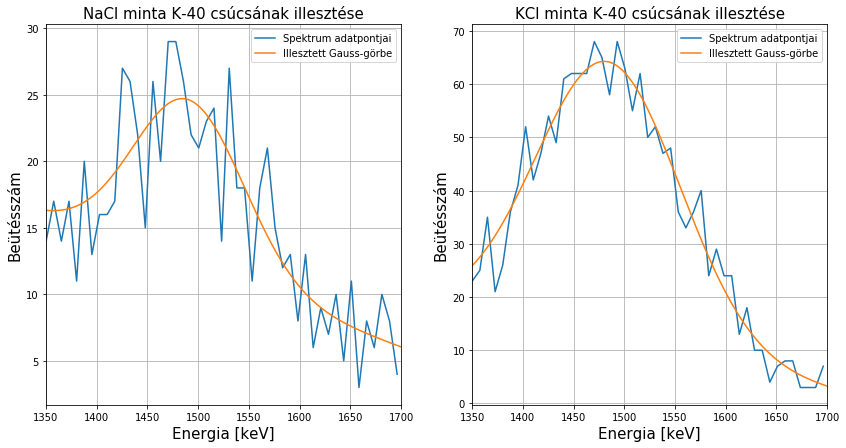
\includegraphics[scale=0.50]{K40_fits}
\caption{NaCl és KCl mintákkal mért $^{40}$K csúcsok és azok illesztései. A NaCl mintával végzett mérés 120 s-ig tartott, kétszer annyi ideig, míg a KCl mintával végzett mérés, így a kapott amplitúdó kétszeresével kell számolni a KCl minta esetében.}
\label{fig:6}
\end{figure}

Az illesztési paramétereket az alábbi táblázat tartalmazza:
\begin{table}[!h]
\begin{center}
\begin{tabular}{|c|c||c|}
\hline
- & NaCl minta & KCl minta \\
\hline
$A$ & $12.712 \pm 1.512$ & $52.755 \pm 2.545$ \\
\hline
$\mu$ [keV] & $1490.893 \pm 7.321$ & $1484.088 \pm 3.195$ \\ 
\hline
$\sigma$ [keV] & $54.592 \pm 9.233$ & $71.317 \pm 4.599$ \\
\hline
$c$ [1/keV] & $-0.028 \pm 0.006$ & $-0.040 \pm 0.010$ \\
\hline
$b$ & $53.731 \pm 9.405$ & $71.363 \pm 17.232$ \\
\hline
\end{tabular}
\caption{$^{40}$K csúcsokra vonatkozó illesztési paraméterek}
\end{center}
\end{table}
\newline
A fentiek alapján a két csúcs intenzitásának, így amplitúdóinak arányát az alábbi módon lehet számolni:
$$\frac{1}{2}\frac{A^{*}_{\textrm{NaCl}}}{A^{*}_{\textrm{KCl}}}=
\frac{A_{\textrm{NaCl}}}{A_{\textrm{KCl}}}\cdot  \frac{\sigma_{\textrm{NaCl}}}{\sigma_{\textrm{KCl}}} = 0.092 \pm 0.012 ,$$
ahol a hibát az egyes tagok relatív hibáinak négyzetösszegével számoltam. Ez a hiba azonban csak az illesztésből származó pontatlanságokat tükrözi, az egyes beütésszámok azonban a független eseményekre vonatkozó Poisson-hibával is terhelve vannak, mely a beütésszámok négyzetgyökének felel meg. Ha ezt is hozzávesszük a fentebb számolt hibához, vagyis a relatív hibát a 
$$\frac{\Delta x}{x} = \sqrt{\sum_{i=\textrm{NaCl,KCl}} \left(\frac{\Delta A_i}{A_i}\right)^2 + \sum_{i=\textrm{NaCl,KCl}} \left(\frac{\Delta \sigma_i}{\sigma_i}\right)^2 + \frac{1}{N_{\textrm{NaCl}}} + \frac{1}{N_{\textrm{KCl}}}} $$
képlet segítségével a fenti érték hibájára $\Delta = 0.017$-et kapunk.
\newpage
\subsection{Félvezető detektor (HPG)}
\hspace*{10pt} A szcintillációs detektorhoz hasonlóan itt is a detektor kalibrálását végezzük el először. Ehhez ugyanazon minták spektrumát vettük fel amiket a szcintillációs detektornál is használtunk. A félvezető detektornál a korábbival ellentétben csak egy spektrumot vettünk fel, a mérés során a mintákat cseréltük ki. A mért spektrum a \ref{fig:7} . ábrán látható.

\begin{figure}[!h]
\centering
\includegraphics[scale=0.60]{HPG}
\caption{A HPG-vel felvett spektrum}
\label{fig:7}
\end{figure}

Az illesztéseket a korábbihoz hasonló módon végeztük. A kobalt csúcsainak illesztése a \ref{fig:8} . ábrán látható.

\begin{figure}[!h]
\centering
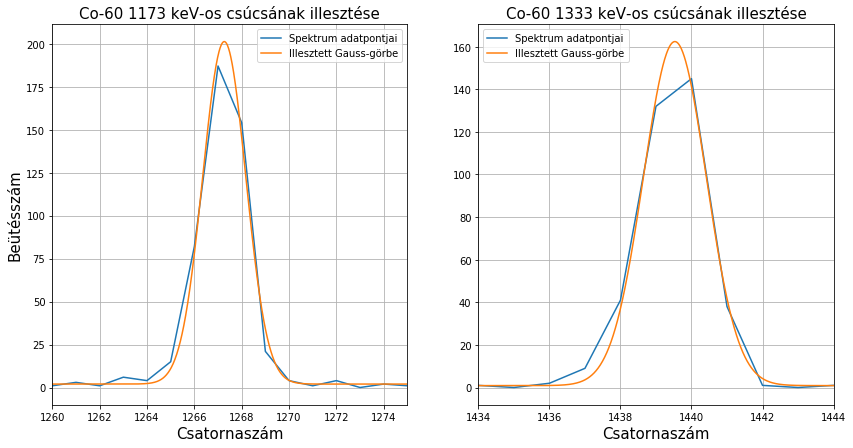
\includegraphics[scale=0.50]{Co_hpg}
\caption{A kobalt első (1173 keV) és második (1333 keV) csúcsának illesztése a HPG-vel felvett spektrum esetén}
\label{fig:8}
\end{figure}

\newpage

Az illesztési paraméterek:

\begin{table}[!h]
\begin{center}
\begin{tabular}{|c|c||c|}
\hline
- & 1173 keV & 1333 keV \\
\hline
$A$ & $199.211 \pm 4.460$ & $161.513 \pm 3.236$ \\
\hline
$\mu$ & $1267.263 \pm 0.023$ & $1439.532 \pm 0.020$ \\ 
\hline
$\sigma$ & $0.909 \pm 0.243$ & $0.886 \pm 0.022$ \\
\hline
$c$ & $2.000 \pm 1.130$ & $0.890 \pm 1.047$ \\
\hline
\end{tabular}
\caption{$^{60}$Co csúcsokra vonatkozó illesztési paraméterek}
\end{center}
\end{table}

A cézium csúcsának illesztése (\ref{fig:9} . ábra):

\begin{figure}[!h]
\centering
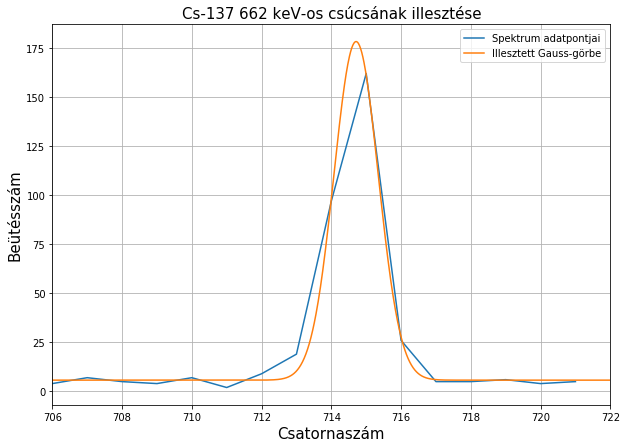
\includegraphics[scale=0.60]{Cs137_1csucs_hpg}
\caption{A cézium csúcsának (662 keV) illesztése}
\label{fig:9}
\end{figure}

Az illesztési paraméterek:
\begin{table}[!h]
\begin{center}
\begin{tabular}{|c|c|}
\hline
Energia & 662 keV \\ 
\hline
$A$ & $172.539 \pm 4.197$\\
\hline
$\mu$ & $714.710 \pm 0.017$\\
\hline
$\sigma$ & $0.636 \pm 0.020$\\
\hline
$c$ & $5.750 \pm 0.894$\\
\hline
\end{tabular}
\caption{A cézium spektrumában látható csúcs illesztési paraméterei}
\end{center}
\end{table}

\newpage

Az illesztési paraméterek segítségével ezen detektor esetében is el tudjuk végezni a kalibrációt, szintén egyenesillesztés segítségével, a fent már kifejtett módon. A kalibrációs egyenes a \ref{fig:10} . ábrán látható.

\begin{figure}[!h]
\centering
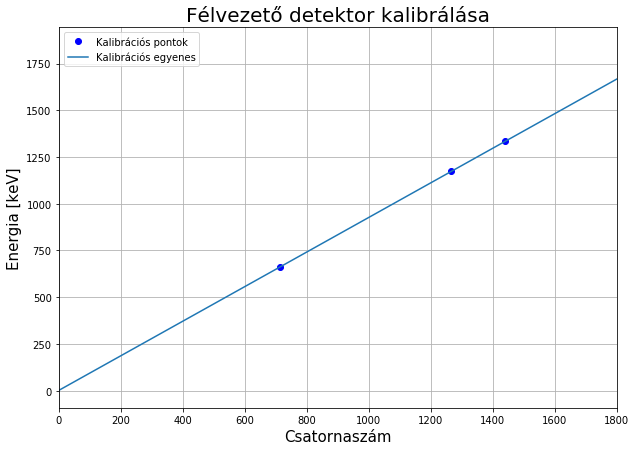
\includegraphics[scale=0.60]{HPG_kalib}
\caption{A félvezető detektor kalibrálásához készített egyenesillesztés}
\label{fig:10}
\end{figure}

A kalibrációs egyenes egyenlete:

$$E(x)=0.926 \cdot x + 0.450$$

A detektor felbontóképességét itt is a $^{60}$Co vonal félértékszélességével írhatjuk le a \ref{fig:4} . ábránál tapasztaltakhoz hasonlóan. Ez alapján a HPG felbontóképességére $\Delta x = (1.935 \pm 0.049)$ keV adódik. Ezen felbontásérték segítségével közelítőleg azonosítani tudunk bizonyos bomlástermékeket a HPG spektrumában. A feladatunk a $^{238}$U három bomlástermékének, a $^{214}$Bi (609.318 keV), $^{214}$Pb (351.9 keV) és a $^{214}$Pb (295.2 keV) csúcsának spektrumon belüli azonosítása volt. Ehhez kivágtuk a spektrum irodalmi energiaérték körüli tartományát, majd a felbontóképességen belül detektálható csúcsot azonosítottuk a keresett leányelemként. A spektrumrészletek és a csúcsok azonosításai a \ref{fig:11} . ábrán látható.
\newpage

\begin{figure}[!h]
\centering
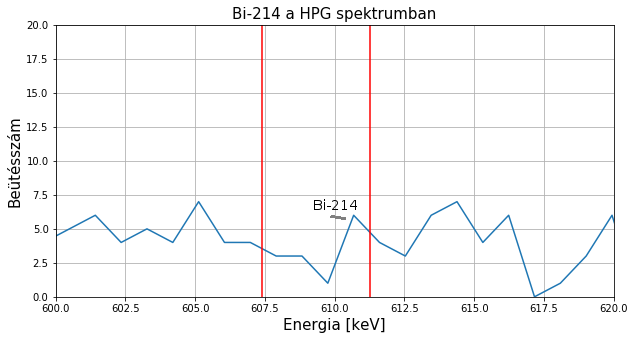
\includegraphics[scale=1]{Bi_csucs}
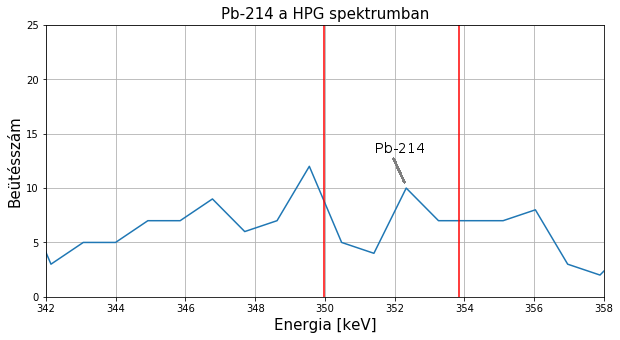
\includegraphics[scale=1]{Pb_csucs}
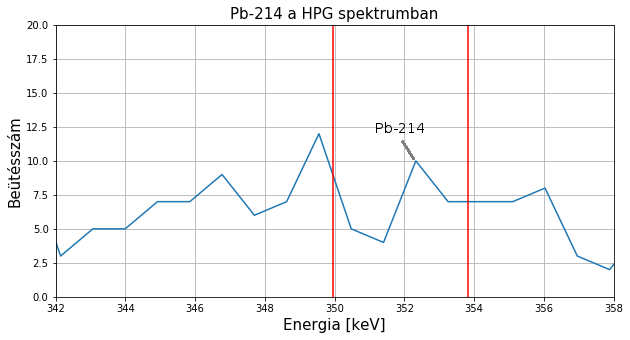
\includegraphics[scale=1]{Pb_2csucs}

\caption{$^{238}$U leányelemeinek azonosítása. A piros sávok a felbontóképességet jelölik, a sávok között félúton az irodalmi energiaértékek helyezkednek el}\label{fig:11}
\end{figure}
\newpage

A választott csúcsok leolvasott energiaértékei az alábbi táblázatban láthatók:
\begin{table}[!h]
\begin{center}
\begin{tabular}{|c|c|c|}
\hline
Izotóp & Irodalmi energia [keV] & Leolvasott energia [keV]\\
\hline
$^{214}$Bi & 609.32 & 610.68\\
\hline
$^{214}$Pb & 351.90 & 352.33\\
\hline
$^{214}$Pb & 295.20 & 296.77\\ 
\hline
\end{tabular}
\caption{A leányelemek leolvasott helyei. A választott csúcsok mind a kontinuum statisztikus ingadozása felett (Poisson-hiba), valamint a felbonthatósági határon belül vannak}
\end{center}
\end{table}

A táblázatban látható irodalmi értékeket a [2]-ból írtam ki. A spektrumokban az ábrákon látható módon fel lehet lelni az urán leányelemei által létrehozott csúcsokat, azonban a pontosabb energiaméréshez és a csúcsok jobban láthatóvá tételéhez hosszabb idejű mérésekre lett volna szükség. 

\end{document}